% ch04-electronics.tex -- Chapter 4: Capacitors, inductors and RC/RL transients
\chapter{Capacitors, inductors and RC/RL transients}
\label{ch:transients}

Chapters 1--3 lived in a world where every voltage settles instantly. Real
circuits don't: they have \emph{memory}, and the two components that carry it
are the capacitor and the inductor. This chapter gives you the one
differential equation this book needs, its famous answer (the exponential,
with time constant $\tau$), and the three places transients actually ambush
you on a bench: switch debouncing, power-up behaviour, and the decoupling
capacitor that guards every chip's supply pin. By the end you can predict a
delay to the millisecond, size an RC for it, simulate the response, and
explain why opening an inductor's circuit is a way to kill a transistor.

\section{The capacitor: charge bucket, $i = C\,dv/dt$}
\label{sec:cap}

A \emph{capacitor}\index{capacitor} is two conductors facing each other
across an insulator. Charge pushed onto one plate repels charge off the
other; the stored charge is $Q = CV$, where the \emph{capacitance}
\index{capacitance} $C$ in farads measures how much charge one volt packs
away. Since current is charge per second, differentiating gives the element
law:
\[
i = C\,\frac{dv}{dt}.
\]
Read it both ways: current \emph{through} a capacitor means its voltage is
\emph{changing}, and a capacitor whose voltage is changing draws or supplies
current proportional to the rate. Two consequences worth memorising now:
capacitor voltage \emph{cannot jump} (a jump would need infinite current),
and at DC a charged capacitor is an open circuit — zero $dv/dt$, zero current.

\begin{figure}[htbp]
\centering
% fig_charge.tex -- Figure 4.1: capacitor as charge bucket
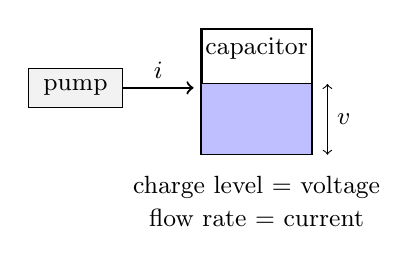
\begin{tikzpicture}
  % battery pumping charge
  \draw[fill=gray!10] (0,0) rectangle (1.2,0.5);
  \node at (0.6,0.25) {\small pump};
  \draw[->,thick] (1.2,0.25) -- (2.1,0.25);
  \node[above] at (1.65,0.25) {\small $i$};
  % bucket
  \draw[thick] (2.2,-0.6) -- (2.2,1.0) -- (3.6,1.0) -- (3.6,-0.6);
  \draw[fill=blue!25] (2.2,-0.6) rectangle (3.6,0.3);
  \draw[<->] (3.8,-0.6) -- (3.8,0.3) node[midway,right]{\small $v$};
  \node at (2.9,0.75) {\small capacitor};
  \node[below,align=center] at (2.9,-0.75) {\small charge level = voltage\\ \small flow rate = current};
\end{tikzpicture}

\caption{The bucket picture. Charge is the water level (voltage), current is
the flow rate, capacitance is the bucket's width. A wide bucket ($C$ big)
fills slowly for the same flow — that is why big capacitors make slow
circuits.}
\label{fig:charge04}
\end{figure}

The stored energy is $E=\tfrac12 CV^2$ — real energy, returned later, which
is what makes capacitors useful for smoothing and why a charged capacitor on
an unplugged board still bites (Section~\ref{sec:safety4}).

\section{The RC step response}
\label{sec:rcstep}

Connect a resistor from a voltage source to an uncharged capacitor
(Figure~\ref{fig:divider} of Chapter~3, second element now a $C$). KCL at the
capacitor node:
\[
\frac{V-v}{R} = C\frac{dv}{dt}
\quad\Longrightarrow\quad
\frac{dv}{dt}+\frac{v}{RC}=\frac{V}{RC}.
\]
This is a first-order linear ODE — the only one this book asks you to derive,
once, in the exercises. Its solution for $v(0)=0$ is
\[
v(t) = V\bigl(1-e^{-t/\tau}\bigr),\qquad \tau = RC,
\]
where $\tau$\index{time constant} — the \emph{time constant} — is the single
number that controls everything. The derivation matters once; the shape
matters forever (Figure~\ref{fig:rcstep}).

\begin{figure}[htbp]
\centering
% fig_rcstep.tex -- Figure 4.2: RC step response, real .tran data
\begin{tikzpicture}
\begin{axis}[width=0.85\textwidth, height=6cm,
  xlabel={$t$ (\unit{\milli\second})}, ylabel={$v_C$ (\unit{\volt})},
  xmin=0, xmax=5, ymin=0, ymax=5.4, grid=both, grid style={gray!15}]
  \addplot[blue, thick] table {figures/ch04/ch04_rc_step_ms.dat};
  \addplot[gray, dashed] coordinates {(0,5) (5,5)};
  \node[font=\small] at (axis cs:3.6,4.55) {$v_C = 5(1-e^{-t/\tau})$};
\end{axis}
\end{tikzpicture}

\caption{Real \texttt{.tran} output of the RC step: \qty{5}{\volt} through
\qty{1}{\kilo\ohm} into \qty{1}{\micro\farad}, so $\tau=\qty{1}{\milli\second}$.
Notice the charging is fastest at the start — the gap between target and
present voltage is what drives the current, so the approach is always
exponential, never linear.}
\label{fig:rcstep}
\end{figure}

\begin{figure}[htbp]
\centering
% fig_tau.tex -- Figure 4.3: tau marked at 63%
\begin{tikzpicture}
\begin{axis}[width=0.85\textwidth, height=6cm,
  xlabel={$t$ (\unit{\milli\second})}, ylabel={$v_C$ (\unit{\volt})},
  xmin=0, xmax=5, ymin=0, ymax=5.4, grid=both, grid style={gray!15}]
  \addplot[blue, thick] table {figures/ch04/ch04_rc_step_ms.dat};
  \addplot[gray, dashed] coordinates {(0,3.162) (1,3.162) (1,0)};
  \addplot[black, only marks, mark=*, mark size=1.8pt] coordinates {(1,3.162)};
  \node[font=\small, anchor=west] at (axis cs:1.15,3.162) {\qty{63}{\percent} at $t=\tau$};
  \node[font=\small] at (axis cs:2.9,1.1) {each $\tau$ erases \qty{63}{\percent} of what is left};
  \addplot[gray, dotted] coordinates {(0,5) (5,5)};
\end{axis}
\end{tikzpicture}

\caption{The number to memorise: at $t=\tau$ the capacitor reaches
\qty{63}{\percent} ($1-e^{-1}$) of its target. Each further $\tau$ closes
\qty{63}{\percent} of the \emph{remaining} gap — at $5\tau$ it is
\qty{99.3}{\percent} there, which is the engineer's ``done''.}
\label{fig:tau}
\end{figure}

\begin{checkpoint}
The sim above uses $R=\qty{1}{\kilo\ohm}$, $C=\qty{1}{\micro\farad}$.
Predict $v_C$ at $t=\qty{2}{\milli\second}$: $5(1-e^{-2})=\qty{4.32}{\volt}$.
The simulation agrees to three figures.
\end{checkpoint}

\section{Charging vs discharging}
\label{sec:chargedis}

Discharge is the mirror image: a charged cap through a resistor to ground
obeys $RC\,dv/dt = -v$, giving $v(t)=V_0 e^{-t/\tau}$ — the same exponential
flipped (Figure~\ref{fig:chargedis}). Charging and discharging are one
phenomenon — exponential approach to a target; only the target differs.

\begin{figure}[htbp]
\centering
% fig_chargedischarge.tex -- Figure 4.4: charging vs discharging
\begin{tikzpicture}
\begin{axis}[width=0.85\textwidth, height=6cm,
  xlabel={$t$ (\unit{\milli\second})}, ylabel={$v_C$ (\unit{\volt})},
  xmin=0, xmax=5, ymin=0, ymax=5.4, grid=both, grid style={gray!15},
  legend style={at={(0.97,0.5)},anchor=east,font=\small}]
  \addplot[blue, thick] table {figures/ch04/ch04_rc_step_ms.dat};
  \addlegendentry{charging toward 5 V}
  \addplot[red, thick] table {figures/ch04/ch04_rc_discharge_ms.dat};
  \addlegendentry{discharging toward 0}
\end{axis}
\end{tikzpicture}

\caption{Same $R$, same $C$, opposite targets — real \texttt{.tran} for both.
Notice the curves are reflections: at $t=\tau$ the charging curve sits at
\qty{63}{\percent} of full and the discharging at \qty{37}{\percent}.}
\label{fig:chargedis}
\end{figure}

\begin{exercise}[easy]
A \qty{1}{\micro\farad} cap charges through \qty{2.2}{\kilo\ohm} toward
\qty{5}{\volt}. Give $\tau$, and the voltage at $t=\tau$ and $t=3\tau$.
(Answer: \qty{2.2}{\milli\second}; \qty{3.16}{\volt}; \qty{4.75}{\volt}.)
\end{exercise}

\begin{example}[A 555-style delay: how long to \qty{3.33}{\volt}?]
\label{ex:delay555}
\textbf{Strategy.} The 555 timer (Chapter~13 territory) trips when its RC
reaches $\tfrac23 V_{CC}$. So the delay question is: for $v(t)=5(1-e^{-t/\tau})$,
solve $v(t^*)=\qty{3.33}{\volt}$.

\textbf{Solution.} $1-e^{-t/\tau}=2/3 \Rightarrow e^{-t/\tau}=1/3
\Rightarrow t^*=\tau\ln 3=1.0986\,\tau$. With $\tau=\qty{1}{\milli\second}$:
$t^*=\qty{1.099}{\milli\second}$.

\textbf{Check.} The \texttt{.tran} data of Listing~\ref{lst:rcstep} crosses
\qty{3.33}{\volt} at \qty{1.10}{\milli\second} — agreement to the third
digit, which is all the precision an electrolytic capacitor deserves.
\end{example}

\begin{lstlisting}[language={},caption={\texttt{code/ch04\_rc\_step.cir} — the step that produces Figures~\ref{fig:rcstep}--\ref{fig:tau} (simulation S1). The discharge twin \texttt{code/ch04\_rc\_discharge.cir} is the same file with the source removed and \texttt{.ic v(2)=5}.},label=lst:rcstep]
* ch04_rc_step.cir -- RC step response: 0->5 V step through R=1k into C=1uF
V1 1 0 PULSE(0 5 0 1n 1n 1 1)
R1 1 2 1000
C1 2 0 1u
.control
tran 5u 5m
let vout = v(2)
set filetype=ascii
wrdata ch04_rc_step.dat vout
.endc
.end
\end{lstlisting}

\begin{lstlisting}[language={},caption={Actual rows of \texttt{ch04\_rc\_step\_ms.dat} (the ms-rescaled file of Figure~\ref{fig:tau}; ngspice's adaptive steps land on these timestamps, not round numbers) — \qty{3.158}{\volt} at \qty{0.999}{\milli\second} is the 63\% mark, and \qty{3.334}{\volt} at \qty{1.099}{\milli\second} is the $\tau\ln 3$ crossing of Example~\ref{ex:delay555}.},label=lst:rcdata]
t(ms)           v(2)
8.988090e-01    2.964732e+00
9.988090e-01    3.158414e+00
1.098809e+00    3.333664e+00
1.198809e+00    3.492237e+00
\end{lstlisting}

\section{The inductor: the dual element}
\label{sec:ind}

The \emph{inductor}\index{inductor} mirrors the capacitor: a coil that stores
energy in its magnetic field and obeys
\[
v = L\,\frac{di}{dt},
\]
dual to $i=C\,dv/dt$\index{inductance}. Its time constant in a resistor
network is $\tau=L/R$\index{time constant!RL} — current through an inductor
cannot jump, and at DC it is a short. We keep it lighter than the capacitor
because its role in this book is mostly a warning label — the next section
shows why.

\begin{exercise}[easy]
An RL circuit has $L=\qty{10}{\milli\henry}$ in series with
$R=\qty{100}{\ohm}$. What is $\tau$, and how long until the current reaches
\qty{95}{\percent} of its final value? (Answer: \qty{100}{\micro\second};
$3\tau=\qty{300}{\micro\second}$.)
\end{exercise}

\section{RL transients and the flyback spike}
\label{sec:flyback}

Energise a coil and its current ramps exponentially toward $V/R$. Now open
the switch mid-current. The inductor's rule is absolute: $di/dt$ stays
finite, so the current \emph{keeps flowing} — and with nowhere to go it
charges whatever stray capacitance exists until the voltage is large enough
to find a path. That voltage is the \emph{flyback spike}\index{flyback}.

\begin{example}[Relay coil opened at \qty{171}{\milli\ampere}]
\label{ex:flyback}
\textbf{Strategy.} Coil \qty{10}{\milli\henry} with \qty{70}{\ohm} winding
resistance on \qty{12}{\volt}: steady current $12/70=\qty{171}{\milli\ampere}$.
Open the switch; the current has only the \qty{100}{\pico\farad} of stray
wiring capacitance to flow into. Energy conservation estimates the peak:
$\tfrac12 Li^2 \approx \tfrac12 Cv^2 \Rightarrow
v_{\mathrm{peak}}\approx i\sqrt{L/C}$.

\textbf{Solution.} $v_{\mathrm{peak}}\approx
0.171\sqrt{10\,\mathrm{m}/100\,\mathrm{p}} = 0.171\times10^{4}
\approx \qty{1.7}{\kilo\volt}$.

\textbf{Check.} Simulation S3 (Listings~\ref{lst:flybackcir},
Figure~\ref{fig:flyback}) peaks at \qty{1646}{\volt} — \qty{96}{\percent} of
the ideal estimate, the rest eaten by the coil resistance. A real bench sees
this as a killed transistor or a switch contact arc; Chapter~5's flyback
diode is the fix.
\end{example}

\begin{lstlisting}[language={},caption={\texttt{code/ch04\_relay\_flyback.cir} — simulation S3. The warning comment in the file is the point of the exercise.},label=lst:flybackcir]
* ch04_relay_flyback.cir -- open a relay coil mid-current, watch the node fly
* WARNING: the spike this produces (~1.7 kV simulated) is what kills
* transistors. The fix is Chapter 5's flyback diode -- do NOT leave the
* inductor's current path open in real hardware. Simulation S3.
* Topology: 12 V -> Rcoil -> node 2 -> coil L -> node 3 -> switch -> gnd
V1 1 0 DC 12
Rcoil 1 2 70
L1 2 3 10m IC=0
S1 3 0 10 0 SW1
Cpar 3 0 100p
Vsw 10 0 PULSE(1 0 1m 1n 1n 1 1)
.model SW1 SW vt=0.5 vh=0.1 ron=1 roff=1e9
.control
tran 500n 1.06m uic
let vnode = v(3)
wrdata ch04_flyback.dat vnode
.endc
.end
\end{lstlisting}

\begin{figure}[htbp]
\centering
% fig_flyback.tex -- Figure 4.5: relay flyback, real .tran data
\begin{tikzpicture}
\begin{axis}[width=0.85\textwidth, height=6.5cm,
  xlabel={$t$ (\unit{\milli\second})}, ylabel={$v_{\mathrm{node}}$ (\unit{\volt})},
  xmin=0.99, xmax=1.03, ymin=-200, ymax=1900, grid=both, grid style={gray!15}]
  \addplot[red, thick] table {figures/ch04/ch04_flyback_ms.dat};
  \addplot[black, only marks, mark=x, mark size=2.5pt] coordinates {(1.0014,1646)};
  \node[font=\small, anchor=west, align=left] at (axis cs:0.992,1500) {peak \qty{1646}{\volt}\\ predicted \qty{1714}{\volt}};
  \node[font=\small, anchor=west] at (axis cs:0.992,850) {switch opens at \qty{1}{\milli\second}};
\end{axis}
\end{tikzpicture}

\caption{Real \texttt{.tran} output: node 3 sits near ground while the switch
conducts, then leaps to \qty{1646}{\volt} in about a microsecond when it
opens. The marked peak is the estimate of Example~\ref{ex:flyback} — within
\qty{4}{\percent}.}
\label{fig:flyback}
\end{figure}

\section{Where transients hide}
\label{sec:hiding}

Three everyday cases, one physics.

\textbf{Debounce.} A mechanical contact bounces for milliseconds; an RC
filter with $\tau$ of a few ms smooths it into one clean edge (used in
Chapter~9's buttons).

\textbf{Power-up reset.} Hold a reset pin low while the rail climbs through
an RC — instant power-on becomes a deliberate delay, which is why chips come
up sane.

\textbf{Decoupling.} Every chip's supply pin gets a \qty{100}{\nano\farad}
capacitor to ground. When the chip gulps current, the wire's own resistance
would let the rail sag; the local capacitor covers the gulp while the supply
catches up. Example~\ref{ex:decouple} makes it quantitative.

\begin{example}[What \qty{100}{\nano\farad} does to a \qty{200}{\nano\second}
gulp]
\label{ex:decouple}
\textbf{Strategy.} Model the supply path as \qty{5}{\volt} through
\qty{10}{\ohm} of wire and trace impedance; the chip draws a
\qty{50}{\milli\ampere} step for \qty{200}{\nano\second}. Without a cap the
rail falls by Ohm's law; with one, the cap supplies the step and loses only
$\Delta v = I\,\Delta t/C$.

\textbf{Solution.} No cap: $\Delta v=50\,\mathrm{mA}\times10\,\Omega
=\qty{0.50}{\volt}$ — a \qty{10}{\percent} sag, enough to corrupt logic.
With \qty{100}{\nano\farad}: $\Delta v=50\,\mathrm{m}\times200\,\mathrm{n}
/100\,\mathrm{n}=\qty{0.10}{\volt}$.

\textbf{Check.} Simulation S2 (Listing~\ref{lst:decouplecir},
Figure~\ref{fig:decouple}): measured dips \qty{0.50}{\volt} and
\qty{0.091}{\volt} — the \qty{10}{\percent} residual is edge-rate, not
arithmetic. Decoupling is why chips don't brown out on their own switching.
\end{example}

\begin{lstlisting}[language={},caption={\texttt{code/ch04\_decouple.cir} — the with-capacitor run; \texttt{ch04\_decouple\_nocap.cir} removes line 5 (simulation S2, both halves).},label=lst:decouplecir]
* ch04_decouple.cir -- rail droop under a 200 ns, 50 mA current step
V1 1 0 DC 5
R1 1 2 10
C1 2 0 100n
I1 2 0 PULSE(0 0.05 0.5u 1n 1n 0.2u 1)
.control
tran 1n 1.5u
let vrail = v(2)
set filetype=ascii
wrdata ch04_decouple_cap.dat vrail
.endc
.end
\end{lstlisting}

\begin{figure}[htbp]
\centering
% fig_decouple.tex -- Figure 4.6: decoupling before/after, real .tran data
\begin{tikzpicture}
\begin{axis}[width=0.85\textwidth, height=6cm,
  xlabel={$t$ (\unit{\micro\second})}, ylabel={rail voltage (\unit{\volt})},
  xmin=0.3, xmax=1.0, ymin=4.35, ymax=5.1, grid=both, grid style={gray!15},
  legend style={at={(0.5,-0.28)},anchor=north,font=\small}]
  \addplot[gray, thick] table {figures/ch04/ch04_decouple_nocap_us.dat};
  \addlegendentry{no capacitor: \qty{0.50}{\volt} dip}
  \addplot[blue, thick] table {figures/ch04/ch04_decouple_cap_us.dat};
  \addlegendentry{with \qty{100}{\nano\farad}: \qty{0.091}{\volt} dip}
\end{axis}
\end{tikzpicture}

\caption{Real \texttt{.tran} data, zoomed to the gulp. Grey: the rail dips
\qty{0.50}{\volt} bare. Blue: \qty{100}{\nano\farad} holds it to
\qty{0.091}{\volt}. The capacitor does not remove the droop — it covers the
time the supply needs to respond.}
\label{fig:decouple}
\end{figure}

\begin{lstlisting}[language={},caption={\texttt{code/ch04\_tran\_csv.py} — the data pipeline: ngspice writes seconds; this rescales to ms/us for the figures. Every curve in this chapter passes through it.},label=lst:trancsv]
rescale("ch04_rc_step.dat",      "../figures/ch04/ch04_rc_step_ms.dat", 1e3, 4)
rescale("ch04_rc_discharge.dat", "../figures/ch04/ch04_rc_discharge_ms.dat", 1e3, 4)
rescale("ch04_decouple_cap.dat", "../figures/ch04/ch04_decouple_cap_us.dat", 1e6, 3)
rescale("ch04_decouple_nocap.dat","../figures/ch04/ch04_decouple_nocap_us.dat", 1e6, 3)
rescale("ch04_flyback.dat",      "../figures/ch04/ch04_flyback_ms.dat", 1e3, 2)
\end{lstlisting}

\begin{exercise}[medium]
A chip gulps \qty{100}{\milli\ampere} for \qty{50}{\nano\second}. Its
\qty{100}{\nano\farad} decoupling cap covers the gulp. How far does the
local rail sag? (Answer: $\Delta v=I\Delta t/C=\qty{0.05}{\volt}$.)
\end{exercise}

\section{$\star$ Driven RLC: why things ring}
\label{sec:rlc}

Optional, on first reading. Put $L$ and $C$ in one loop and their energies
trade back and forth — the capacitor pushes current that the inductor refuses
to stop, overshooting the target and oscillating at
$\omega_0=1/\sqrt{LC}$\index{ringing}. Resistance bleeds the oscillation
(``damping''); light damping leaves the bell-ringing you saw in
Figure~\ref{fig:flyback}'s spike. That is the whole story: flyback spikes,
switching noise, and every ``why is my square wave wiggly'' are this
exchange, at different $LC$. Chapter~6 uses $\omega_0$; the exercise asks you
to estimate it.

\section{Safety notes}
\label{sec:safety4}

\begin{rulebox}[Capacitors keep their charge]
A capacitor stores energy \emph{after} the power is off. Big electrolytics
can hold a painful voltage for hours — on any board, discharge large caps
through a resistor before touching. This book stays under \qty{9}{\volt}, but
the habit transfers.
\end{rulebox}

\begin{rulebox}[Never leave an energised inductor open]
Example~\ref{ex:flyback} is not decoration: \qty{1.6}{\kilo\volt} from a
\qty{12}{\volt} relay coil. Real hardware switches coils through a
transistor — always with the flyback diode of Chapter~5 fitted, or the
transistor dies on the first off-transition.
\end{rulebox}

\section{Common mistakes}
\label{sec:mistakes4}

\begin{tripwire}[Expecting instant capacitor behaviour]
``It is just a wire when charged'' — true at DC, false during the approach.
If a circuit misbehaves in the first milliseconds, suspect the RC that
settled slower than you assumed.
\end{tripwire}

\begin{tripwire}[Sign errors in the discharge direction]
$v(t)=V_0 e^{-t/\tau}$ decays toward \emph{whatever the capacitor discharges
through}, not always ground. Discharging into a held voltage heads toward
that voltage. Write the ODE, or at least name the target, before the
exponential.
\end{tripwire}

\begin{tripwire}[Steady-state formulas mid-transient]
$V=IR$ and the divider rule describe where the circuit \emph{ends}, not what
it does on the way. During a transient the only honest tools are the element
laws ($i=C\,dv/dt$, $v=L\,di/dt$) and KCL/KVL — as the flyback spike proves
with interest.
\end{tripwire}

\begin{tripwire}[Forgetting inductor current cannot jump]
The inductor's mirror-image rule of the capacitor's. Open an inductor's path
abruptly and physics opens it for you — at kilovolts. Always give inductive
current somewhere to go.
\end{tripwire}

\section{Chapter summary}
\label{sec:ch4summary}

\begin{table}[htbp]
\centering\small
\begin{tabularx}{\linewidth}{@{}lY l@{}}
\toprule
\thead{Element / idea} & \thead{The one-line version} & \thead{Number} \\
\midrule
Capacitor & current $\Leftrightarrow$ voltage \emph{changes}; $i=C\,dv/dt$ & $Q=CV$, $E=\tfrac12 CV^2$ \\
RC step & exponential approach to target & $\tau=RC$; 63\% at $\tau$, 99\% at $5\tau$ \\
Delay & time to threshold $v_T$ from $V$: $t=\tau\ln\!\frac{V}{V-v_T}$ & 555-style $\tfrac23$: $1.099\,\tau$ \\
Inductor & voltage $\Leftrightarrow$ current \emph{changes}; $v=L\,di/dt$ & $\tau=L/R$ \\
Flyback & opened inductor: $v_{\mathrm{pk}}\approx i\sqrt{L/C}$ & \qty{1.6}{\kilo\volt} from 12 V here \\
Decoupling & local cap covers $\Delta t$ gulps: $\Delta v=I\Delta t/C$ & \qty{100}{\nano\farad} per chip pin \\
Uses & debounce $\tau\sim$ms; reset delay; supply smoothing & real circuits in Part II \\
\bottomrule
\end{tabularx}
\caption{Chapter 4 on a page. Everything here is one idea — exponential
approach — applied to two dual elements.}
\label{tab:ch4summary}
\end{table}

\begin{wins}
\begin{itemize}
\item You can derive the RC step response, read any exponential's $\tau$, and
estimate delays and dips to first order.
\item You know why capacitors sit on supply pins, why contacts need
debouncing, and why reset lines exist.
\item You have watched an inductor make \qty{1.6}{\kilo\volt} from 12 V — and
you know the diode chapter is coming.
\item Every curve you saw is real \texttt{.tran} output you can regenerate
from \texttt{code/ch04\_*.cir}.
\end{itemize}
\end{wins}

\section*{Exercises}
\addcontentsline{toc}{section}{Exercises}

\begin{exercise}[easy]
$\tau$ for (a) $R=\qty{4.7}{\kilo\ohm},C=\qty{10}{\micro\farad}$; (b)
$R=\qty{330}{\ohm},C=\qty{100}{\nano\farad}$; (c) $R=\qty{10}{\kilo\ohm},
L=\qty{100}{\milli\henry}$ (RL).
\end{exercise}

\begin{exercise}[easy]
Charging from 0 toward \qty{9}{\volt} through $\tau=\qty{5}{\milli\second}$:
what is $v_C$ at $t=\qty{5}{\milli\second}$, \qty{10}{\milli\second},
\qty{25}{\milli\second}?
\end{exercise}

\begin{exercise}[easy]
A \qty{10}{\micro\farad} cap charged to \qty{5}{\volt}: how much charge and
energy does it hold?
\end{exercise}

\begin{exercise}[easy]
Two \qty{10}{\micro\farad} caps (a) in parallel, (b) in series: give
$C_{\mathrm{eq}}$ each way — and which arrangement would you pick for a
bigger decoupling reservoir?
\end{exercise}

\begin{exercise}[medium]
A 555-style trigger needs \qty{2.5}{\volt} from a \qty{9}{\volt} rail. Using
the step-response formula, what $t/\tau$ ratio is the delay?
\end{exercise}

\begin{exercise}[medium — derive]
Derive the step response from the ODE: separate variables in
$RC\,dv/dt = V-v$, integrate from $(0,0)$ to $(t,v)$, and confirm
$v=V(1-e^{-t/\tau})$. Then differentiate back to find $i(t)$ — is it
largest at $t=0$? Why physically?
\end{exercise}

\begin{exercise}[medium — design]
You need a power-on delay of about \qty{50}{\milli\second} before a reset
releases, using a \qty{10}{\micro\farad} capacitor and the $\tfrac23 V_{CC}$
threshold of Example~\ref{ex:delay555}. Pick an E24 resistor and report the
achieved delay.
\end{exercise}

\begin{exercise}[medium]
A \qty{100}{\milli\henry} coil with \qty{100}{\ohm} winding resistance is cut
off at its \qty{120}{\milli\ampere} steady current; only
\qty{50}{\pico\farad} of stray capacitance exists. Estimate the flyback peak
— then compare with the safety rulebox.
\end{exercise}

\begin{exercise}[hard]
Write the netlist for discharge \emph{into a held level}: a
\qty{1}{\micro\farad} cap at \qty{5}{\volt} connected at $t=0$ through
\qty{1}{\kilo\ohm} to a \qty{2}{\volt} source. Predict $v_C(t)$ and the
settled value by writing the ODE, then confirm by simulation.
\end{exercise}

\begin{exercise}[hard]
Estimate the ringing frequency if the Example~\ref{ex:flyback} coil
(\qty{10}{\milli\henry}) saw \qty{100}{\pico\farad}: $f_0=1/(2\pi\sqrt{LC})$.
Compare with the sim's spike shape, and say in one sentence why more stray
capacitance would \emph{lower} both the peak voltage and the frequency.
\end{exercise}

\begin{rulebox}[Watch instead]
\begin{itemize}
\item \emph{Capacitors and capacitance} (Khan Academy, 5:43) --- charge stored between plates, and why a capacitor resists sudden voltage change. \url{https://youtu.be/u-jigaMJT10} Listed in Book 8 (ch11), accessed 2026-10-11.
\end{itemize}
\end{rulebox}

\section*{Hints and answers}
\addcontentsline{toc}{section}{Hints and answers}

\begin{description}
\item[$\tau$ values.] (a) \qty{47}{\milli\second}; (b) \qty{33}{\micro\second};
(c) $L/R=\qty{1}{\milli\second}$.
\item[9 V charging.] $9(1-e^{-1})=\qty{5.69}{\volt}$;
$9(1-e^{-2})=\qty{7.78}{\volt}$; $9(1-e^{-5})=\qty{8.94}{\volt}$.
\item[Charge/energy.] $Q=50\,\mu$C; $E=\tfrac12(10\mu)(25)=\qty{125}{\micro\joule}$.
\item[Two caps.] Parallel adds: \qty{20}{\micro\farad}; series halves:
\qty{5}{\micro\farad} — opposite of resistors. For a bigger reservoir pick
parallel (it also halves the effective series resistance, which is the real
reason arrays appear on boards).
\item[2.5 V threshold.] $v/V=0.278 \Rightarrow t/\tau=-\ln(1-0.278)=0.325$.
\item[Derivation.] $\int\frac{dv}{V-v}=\int\frac{dt}{RC}$ gives
$-\ln(V-v)+\ln V=t/RC$, i.e.\ $V-v=Ve^{-t/\tau}$. Then
$i=C\,dv/dt=(V/R)e^{-t/\tau}$ — largest at $t=0$ because the gap (and hence
the resistor voltage) is largest then.
\item[50 ms design.] Need $\tau=50\,\mathrm{ms}/\ln 3=45.5$ ms; with
$C=\qty{10}{\micro\farad}$, $R=4.55\,\mathrm{k}\Omega\to\qty{4.7}{\kilo\ohm}$
E24 gives $\tau=47$ ms, delay $\approx\qty{51.7}{\milli\second}$
(\qty{+3}{\percent} — fine for reset).
\item[Second flyback.] $v_{\mathrm{pk}}\approx0.12\sqrt{100\,\mathrm{m}/50\,\mathrm{p}}
=0.12\times4.47\times10^{4}\approx\qty{5.4}{\kilo\volt}$ — the diode is not
optional.
\item[Discharge into 2 V.] ODE: $RC\,dv/dt=2-v$; solution
$v=2+3e^{-t/\tau}$, settling at \qty{2}{\volt} — the sim agrees; the target
is the \emph{source's} voltage, not zero (the second tripwire in action).
\item[Ringing.] $f_0=1/(2\pi\sqrt{10^{-2}\cdot10^{-10}})\approx
\qty{159}{\kilo\hertz}$ — a few microseconds per cycle, matching the sim's
sharp edge; more $C$ means more charge to absorb the energy (lower
$\sqrt{L/C}$) and a slower exchange (lower $f_0$).
\end{description}

\chapternotes
\begin{enumerate}
\item RC/RL order of topics follows Kuphaldt Vol.~I ch.~13--16 \cite{aacvol1}
(element law, then step response, then applications); the charge-bucket
figure and the 63\% convention are the standard ones.
\item The decoupling model (rail impedance + current gulp) follows the 6.002
sequence of transient-first teaching \cite{ocw6002}; our numbers are chosen
for legibility, not vendor data.
\item Flyback energy argument ($v\approx i\sqrt{L/C}$) and the switch model
are reproduced faithfully by ngspice-47 \cite{ngspice}; real coils differ
mostly in stray capacitance, which only moves the peak, not the physics.
\item Debounce/reset/decoupling placements mirror the applications sections
of \cite{aacvol1}; the diode fix is deferred to Chapter~5 as the plan's hook.
\end{enumerate}
